\section{Características Construtivas}

\subsection{D-MOSFET}

\begin{frame}

    \frametitle{Estrutura}

    \begin{figure}[!htbp]
        \centering
        \caption{Visão em corte vertical de um D-MOSFET}
        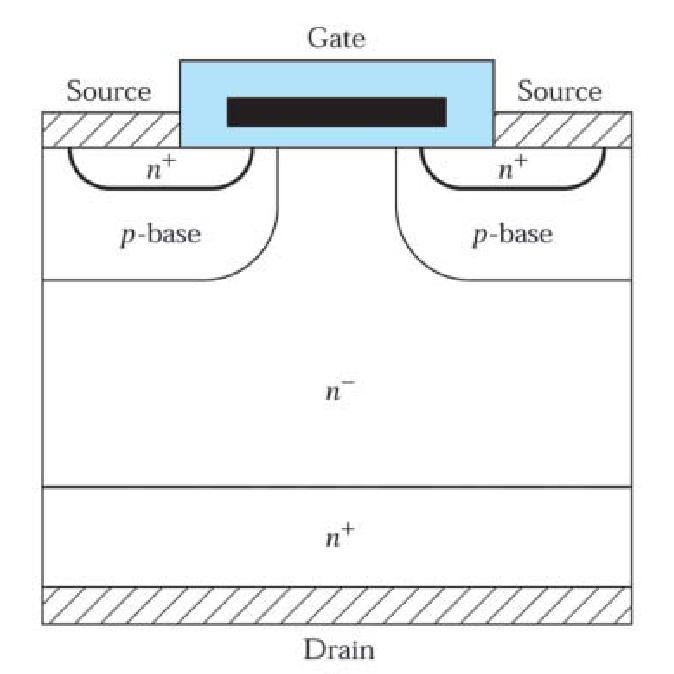
\includegraphics[scale=0.2]{imagens/dmos.png}
        \\\small{\textbf{Fonte:} \cite{sze2012semiconductor}}%
    \end{figure}

\end{frame}

\begin{frame}

    \frametitle{V\textsubscript{blocking}}

    V\textsubscript{blocking} é, principalmente, definida pela região \textit{n\textsuperscript{-}}, chamada de \textit{n-drift}.

    \begin{figure}[!htbp]
        \centering
        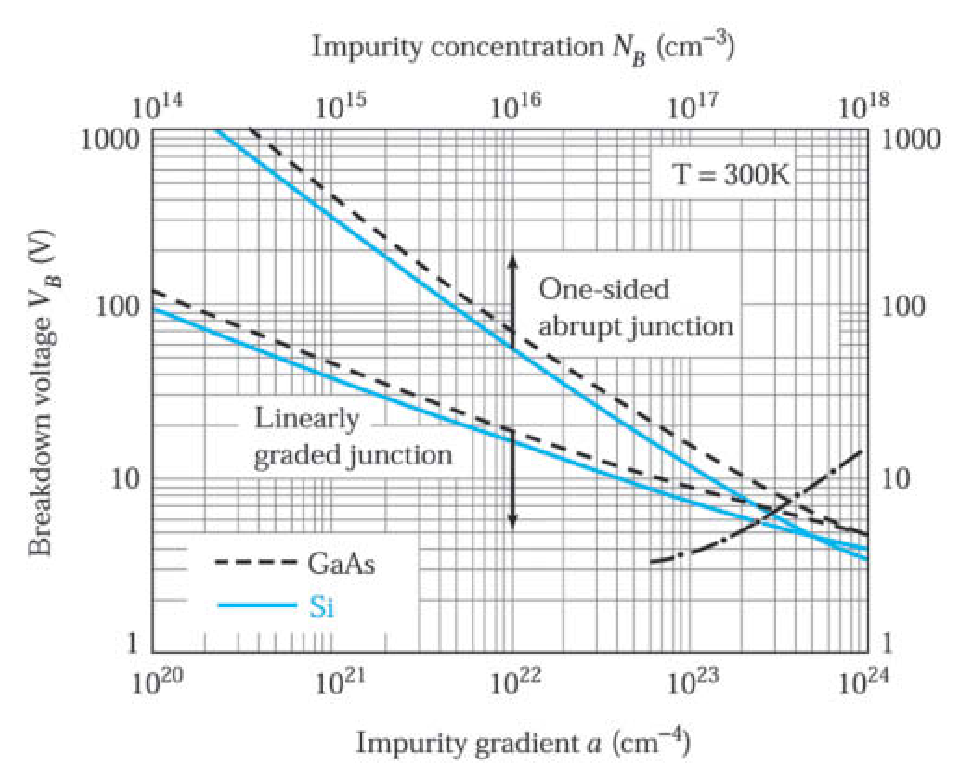
\includegraphics[scale=0.2]{imagens/vblockndrift.png}
        \\\small{\textbf{Fonte:} \cite{sze2012semiconductor}}%
    \end{figure}

\end{frame}

\begin{frame}
    
    \frametitle{R\textsubscript{on}}

    \begin{figure}[!htbp]
        \centering
        \caption{Modelo de composição da resistência de condução de um D-MOSFET}
        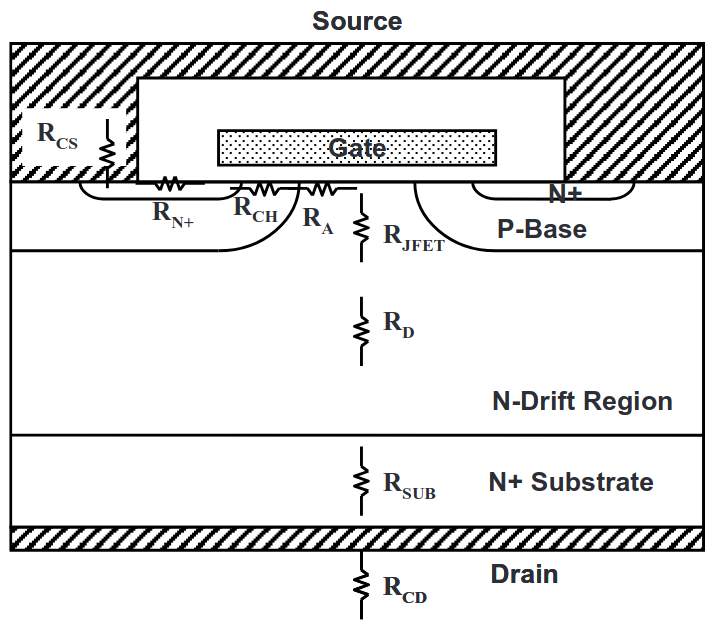
\includegraphics[scale=0.2]{imagens/rondmos_association.png}
        \\\small{\textbf{Fonte:} \cite{baliga2010fundamentals}}%
    \end{figure}

\end{frame}

\begin{frame}
    
    \frametitle{R\textsubscript{on}}

    \begin{figure}[!htbp]
        \centering
        \caption{Cotas relevantes para a resistência de condução de um D-MOSFET}
        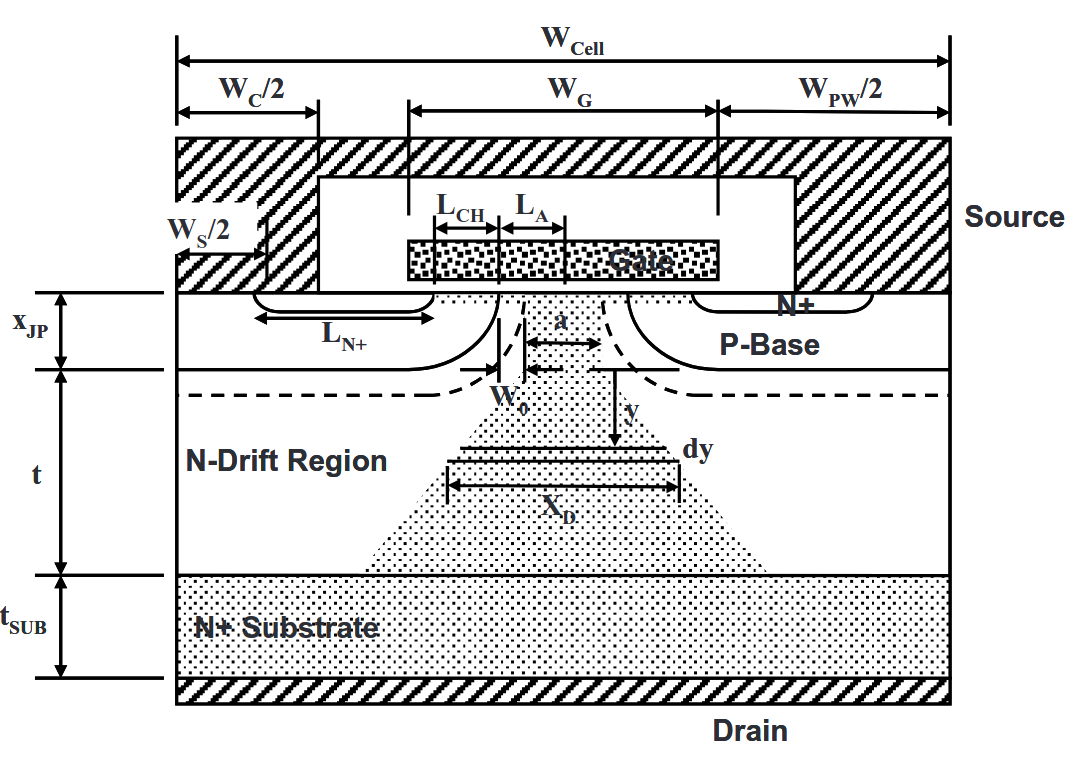
\includegraphics[scale=0.2]{imagens/rondmos_geometry.png}
        \\\small{\textbf{Fonte:} \cite{baliga2010fundamentals}}%
    \end{figure}

\end{frame}

\begin{frame}
    
    \frametitle{R\textsubscript{on}}

    \begin{figure}[!htbp]
        \centering
        \caption{Contribuição dos componentes de R\textsubscript{on} em um D-MOSFET}
        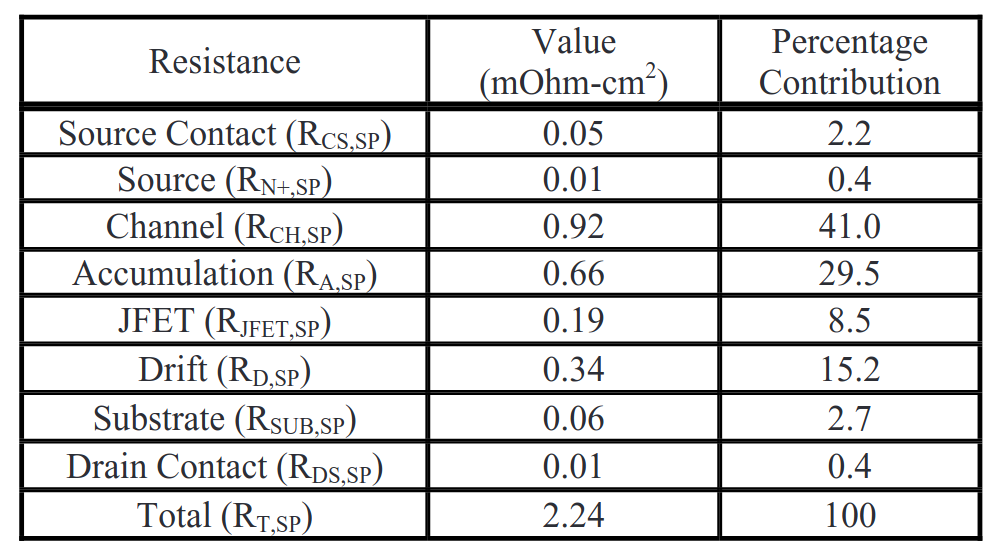
\includegraphics[scale=0.2]{imagens/rondmos_contribution.png}
        \\\small{\textbf{Fonte:} \cite{baliga2010fundamentals}}%
    \end{figure}

\end{frame}

\begin{frame}
    
    \frametitle{R\textsubscript{ch}}

    \begin{equation}
        R_{ch} = \frac{L_{ch}W_{cell}}{2\mu_{ni}C_{ox}(V_G-V_{th})}
    \end{equation}\small{\textbf{Fonte:} \cite{baliga2010fundamentals}}\\

\end{frame}

\begin{frame}

    \frametitle{R\textsubscript{A}}

    \begin{equation}
        R_{A} = K_A\frac{(W_G-2)W_{cell}}{2\mu_{ni}C_{ox}(V_G-V_{th})}
    \end{equation}\small{\textbf{Fonte:} \cite{baliga2010fundamentals}}\\

\end{frame}

\begin{frame}

    \frametitle{R\textsubscript{drift}}

    Multiplos modelos, mas, sempre,

    \begin{gather}
        R_{drift} \propto \rho_D \\ \ \\
        \rho_D = \frac{1}{q(n_D\mu_{n_D} + p_D\mu_{p_D})}
    \end{gather}

\end{frame}
